%=====================================================================
\section{Data}
\label{sec:data}
We use one network per type, chosen to differ in edge meaning, generating mechanism and time scale (seconds, seconds, years); data cards are in \cref{tab:data} and activity time series in \cref{fig:activity}.

\begin{table}[t]
\centering
\small
\setlength{\tabcolsep}{3pt}
\begin{tabular}{@{}llrrll@{}}
\toprule
Type & Dataset & $N$ & Events & Span & Res. \\
\midrule
Contact & Primary school (PS) & 242 & 125\,773 & 2 d & 20 s \\
Comm. & CollegeMsg (CM) & 1\,899 & 59\,835 & 193 d & 1 s \\
Citation & DBLP--DB (CIT) & 19\,150 & 73\,269 & 50 yr & 1 yr \\
\bottomrule
\end{tabular}
\caption{Data cards. $N$: nodes; Res.: temporal resolution. CIT spans publication years 1970--2020, with primary analysis in 1990--2020. PS: undirected, class labels, CC BY-NC-SA;
CM: directed, no labels; CIT: directed, acyclic.}
\label{tab:data}
\end{table}

\paragraph{Face-to-face contact.}
The primary-school data \citep{stehle2011high,gemmetto2014mitigation} were collected by
the SocioPatterns collaboration with wearable proximity sensors over two school days.
A contact is recorded when two people are face to face within about 1.5\,m for at
least 20\,s. Each individual carries a class label, which we use as ground truth for
communities. The data are released under CC BY-NC-SA.

\paragraph{Online communication.}
CollegeMsg \citep{panzarasa2009patterns} contains time-stamped private messages
between 1\,899 users of an online student community over 193 days at 1\,s
resolution. Edges are directed, and there are no node labels.

\paragraph{Scientific publications.}
% Owner: B (measured CIT data card).
We use AMiner DBLP-Citation V14 \citep{tang2008arnetminer}, selected by a fixed
set of database venue families and their declared name variants. Streaming
5,259,858 records yields 19,150 publications from 1970--2020 and 73,269 distinct
citations to strictly older selected papers. These are within-subgraph citations,
not global citation counts; 6,709 nodes are isolates. We save 5,486 same-year
references separately, exclude 6,390 later-year references and 494 self-loops,
and remove 37,440 repeated reference entries. The graph is acyclic under the
strict year rule. AMiner specifies research use; no additional open-data licence
is inferred. The recent fall in observed references despite growing paper counts
motivates a cutoff-2015 sensitivity check and cautions about coverage and censoring.

\paragraph{Preprocessing.}
All data are converted to a common event format $(u,v,t)$ with integer time stamps
(seconds or years) plus a table of node labels. Self-loops and exact duplicate
events are removed, and the first and last partial windows are trimmed. Each source
has known limits: citation data have year-level resolution, the contact data cover only
two days, and the sensors sample only participants who wear them. The three datasets
differ in edge meaning (proximity, message, citation), directedness and time scale
by design, so that agreement across them is not an artefact of one data type.

\begin{figure*}[t]
\centering
\figph{0.46\textwidth}{1.7cm}{PS: events per hour\\Pending A's measured series}\hfill
\figph{0.46\textwidth}{1.7cm}{CM: events per hour\\Pending A's measured series}
\par\medskip
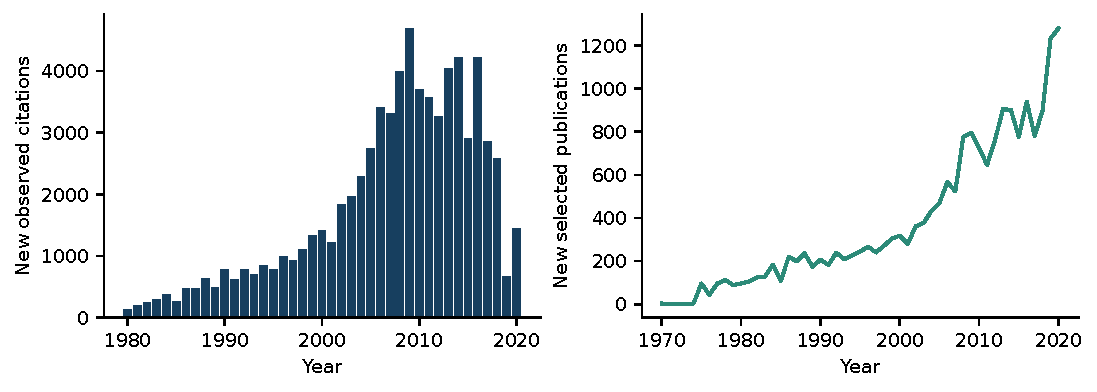
\includegraphics[width=.95\textwidth]{b_activity.pdf}
\caption{Activity overview. The lower panels are measured CIT annual citations
and selected publications; upper panels reserve the pending PS/CM series.
CIT's late reference decline alongside rising publication counts motivates
coverage and observation-cutoff checks.}
\label{fig:activity}
\end{figure*}
